% document formatting
\documentclass[10pt]{article}
\usepackage[utf8]{inputenc}
\usepackage[left=1in,right=1in,top=1in,bottom=1in]{geometry}
\usepackage[T1]{fontenc}
\usepackage{xcolor}

% math symbols, etc.
\usepackage{amsmath, amsfonts, amssymb, amsthm}

% lists
\usepackage{enumerate}

% images
\usepackage{graphicx} % for images

% code blocks
\usepackage{minted, listings} 

% verbatim greek
\usepackage{alphabeta}

\graphicspath{{./assets/images}}

\newcommand{\solution}{\textbf{Solution:}} 
\newcommand{\example}{\textbf{Example: }}
\newcommand{\R}{\mathbb{R}}

\title{BIOMATH 208 Week 1}

\author{Aidan Jan}
\date{\today}

\begin{document}
\maketitle
\section*{Logistics}
\subsection*{Office Hours: Tuesdays 1-3pm}
\subsection*{No midterm/final}
\subsection*{Grading: 80\% homework, 20\% final project}
\section*{Overview}
\begin{enumerate}
    \item Representing and visualizing imaging data
    \begin{itemize}
        \item Pixels, vectors, etc.
    \end{itemize}
    \item Multilinear Algebra
    \begin{itemize}
        \item Linear algebra with stuff added on top
        \item Two types of square matrices
    \end{itemize}
    \item Curves and surfaces
    \begin{itemize}
        \item Comparing curves and surfaces using multilinear algebra
    \end{itemize}
    \item Manifolds
    \item Transformation Groups
    \begin{itemize}
        \item Understanding rotation, linear transformations
    \end{itemize}
    \item Tangent spaces
    \item Optimization and image registration
    \begin{itemize}
        \item Aligning multiple images of the same object
    \end{itemize}
    \item Metric manifolds
    \begin{itemize}
        \item Finding distance between two rotation matrices, ellipsoids, probabilities, etc.
        \item Using distances to compute averages, make predictions, etc.
    \end{itemize}
    \item Averaging filtering and regression
\end{enumerate}

\section*{Representing images}
\begin{itemize}
    \item Definition (images): We generally consider images as functions from some set $X \subseteq \mathbb{R}^d$, to some other set, $S$.
    \begin{itemize}
        \item $X$ describes space; usually, $d = 2$ or $d = 3$, depending on the dimension of the image.
    \end{itemize}
    \item What this means:
    \begin{itemize}
        \item Let $X$ represent a picture, some 2D set of pixels in this example.  Let $x \subset X$, where $x$ is a pixel in the picture.
        \item We can define the image, $I$, as a function, such that $X \::\: X \rightarrow S$, where $S$ is a pixel value.
        \begin{itemize}
            \item $S \in \R$ if the image is grayscale, and $S \in R^3$ if the image is colored.
        \end{itemize}
    \end{itemize}
\end{itemize}

\subsubsection*{Example 1}
\begin{center}
    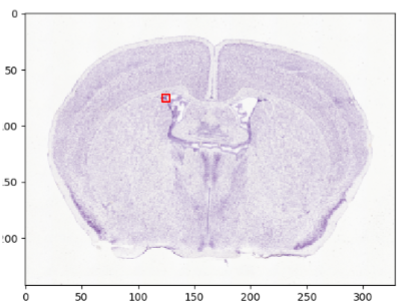
\includegraphics[scale=1]{W1_1.png}
\end{center}
\begin{itemize}
    \item Above is a microscopy image of a Nissl stained mouse brain.
    \item Here, $d = 2$ with $X$ some rectangle, and $S = [0, 1]^3$ containing $3$ RGB values, each value between 0 and 1.
\end{itemize}

\subsubsection*{Example 2}
\begin{center}
    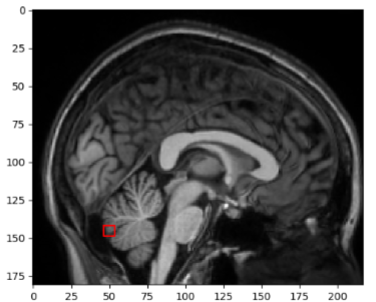
\includegraphics[scale=1]{W1_2.png}
\end{center}
\begin{itemize}
    \item Above is a part of a human brain MRI.  The set $X$ is shown on the axes.
    \item Here, $d = 3$, since this is a 3D image.  $S = \R$ since it is grayscale, therefore only one value.
    \begin{itemize}
        \item The $S$ value is a value between $[0, 1]$ representing the brightness of the pixel.
    \end{itemize}
\end{itemize}

\subsubsection*{Example 3 - Label Images}
\begin{center}
    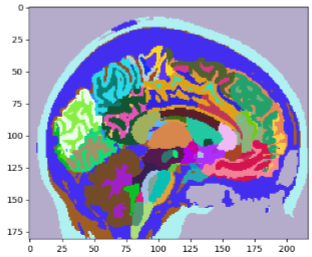
\includegraphics[scale=1]{W1_3.png}
\end{center}
\begin{itemize}
    \item Here, $d = 3$ with $X$ some rectangular prism, and $S = \mathbb{N}$ containing 1 integer, \texttt{id}.  Each \texttt{id} represents some particular type of structure.  
    \item Part of a labeled brain image is shown.  Integers are shown as colors, and the set $X$ is shown on the axes for one slice of the 3D volume.
\end{itemize}

\subsection*{Discrete Images}
\begin{itemize}
    \item Treating images as functions is nice, because they have basically infinite resolution.  (You can plug in any coordinate value and receive the corresponding values.)
    \item However, we can't store the functions in a computer.  As a result, we usually work with \textbf{discrete images}.
    \item In this case, images are $d$-dimensional arrays, storing values in $S$.
    \begin{itemize}
        \item Geometry is stored with pixel size $\Delta \in \R^d$, and origin $O \in \R^d$.
        \item Square brackets are used to index starting from 0. \texttt{img[0, 0]} would represent the top left corner.
        \item In 3D, we would use rows, columns, and slices.
        \item We may also specify the location of the origin, $O$, to scale in real life.  Origin is \texttt{img[0, 0]}, but may be assigned some real world location, for example, [10ft, 20ft].  $\Delta$ is the pixel size, and therefore the physical location for any pixel can be calculated.  (Real location of pixel \texttt{img[i,j]} would be $O + \Delta \cdot {i \choose j}$).
    \end{itemize}
\end{itemize}

\subsection*{Grayscale images}
\begin{center}
    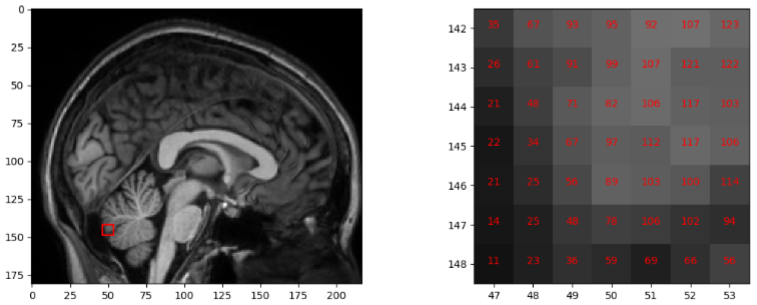
\includegraphics[scale=1]{W1_4.png}
\end{center}
\begin{itemize}
    \item Here we see a sagittal view of a brain MR image, and a zoom in showing pixel values.
    \item Here, the origin is (0, 0), and the spacing is (1, 1) (in mm).
\end{itemize}

\subsection*{Color Histology}
\begin{center}
    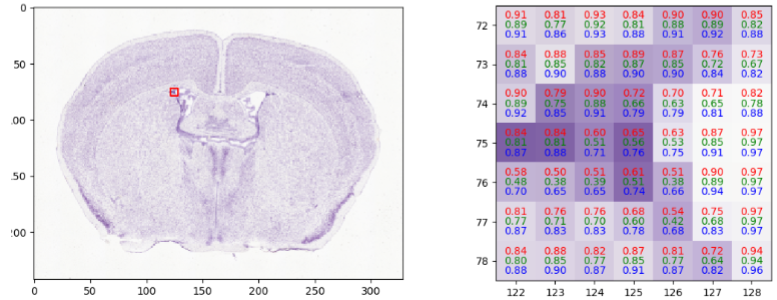
\includegraphics[scale=1]{W1_5.png}
\end{center}
\begin{itemize}
    \item Here we see an image, and a zoom in showing pixel values as RGB triples.
    \item Here the origin is (0, 0), and the spacing is (58.8, 58.8) (in microns).
\end{itemize}

\section*{Interpolation}
Interpolation links images as functions to images as discrete arrays.  If $S$ is a vector space, then we can specify an interpolation kernel $h$ and write
\[I(x) = \sum_{i, j, k} I[i, j, k] h(x - x[i, j, k])\]
where $x[i, j, k] = O + \text{diag}(\Delta)\begin{pmatrix} i \\ j \\ k \end{pmatrix}$, the coordinate of the $i, j, k$-th pixel.
\begin{itemize}
    \item $I(x)$ is the image function, and $I[i, j, k]$ is the array of pixels.  $h$ is often a function that is close to 1 near the origin and decays down to zero as you get far away.  
    \begin{itemize}
        \item $h()$ is also known as a point-spread function (psf), or an impulse response function.
    \end{itemize}
    \item What the function basically does is that it multiplies the pixel value by the impulse response function at that real-world location.
    \item We are convolving the kernels with the discrete pixel dataset.  Triangle kernel gives linear interpolation, and rectangle kernel gives nearest neighbor interpolation.
\end{itemize}
\begin{center}
    \includegraphics*[scale=1]{W1_6.png}
    \includegraphics*[scale=1]{W1_7.png}
\end{center}
\begin{itemize}
    \item The image on the left is a brain interpolated (convolved) using the rectangle kernel
    \item The middle image is one interpolated with the triangle kernel
    \item The right image is a brain interpolated with a piecewise cubic function (aka. third degree spline).
\end{itemize}
Importantly, the range of values the function takes is the same as the values.  Since the kernel function is always between values 0-1, the minimum value of the interpolated image is 0, and the maximum is the highest original pixel value.

\subsection*{2D grayscale images}
\begin{itemize}
    \item To display images, intensity values at each pixel need to be mapped to a brightness value on the screen (a number between 0 and 1)
    \item A piecewise linear function is used to do this, by selecting a lower value for black, and an upper value for white.
    \item A histogram of pixel values can be used to choose these parameters.
\end{itemize}
\begin{center}
    \includegraphics*[scale=1]{W1_8.png}
\end{center}
\begin{itemize}
    \item The histogram is one that shows pixel values.  The center should be set at the highest peak of the contrast map, e.g., setting brightness and contrast.
    \item The brightness value is essentially "which pixel value should be mapped to black", and contrast is the "difference between white pixel and black pixel" or, "what pixel value is white relative to black".
    \item The above image sets black to 0 HU, and white to 80 HU.  Anything below the range is black, anything above is white.
\end{itemize}
\subsection*{Summary so far:}
\begin{itemize}
    \item Why study medical images from a geometric point of view?
    \begin{itemize}
        \item Different ways to look at images of the same thing
        \item Looking at the pixel values as a list of numbers is not ideal
        \item Lists of numbers will be called "coordinates"; we want to study in a way that is independent of choice of coordinates
        \item Differential geometry studies this problem.
    \end{itemize}
    \item Images as functions: $I \::\: X \rightarrow S$, where
    \begin{itemize}
        \item $X$ is some subset of space, e.g., inside the scanner
        \item $S$ are the values that pixels might take
        \begin{itemize}
            \item $\R \rightarrow$ grayscale images
            \item $[0, 1]^2 \rightarrow$ colored images
        \end{itemize}
    \end{itemize}
    \item Discrete images
    \begin{itemize}
        \item Two parts:
        \begin{itemize}
            \item An array that stores a set of values ($I[i, j, k]$, if $X \subseteq \R^3$)
            \item An origin and pixel size, $O, \Delta$.  $x[i, j, k] = \begin{pmatrix}
            O^0 + i \Delta^0 \\ O^1 + i \Delta^1 \\ O^2 + i \Delta^2
            \end{pmatrix}$
        \end{itemize}
    \end{itemize}
    \item Interpolation
    \[I(a) = \sum_{i, j, k} \cdot h(x - x[i, j, k])\]
    \begin{itemize}
        \item $h$ is the interpolation kernel.
        \item If $h$ is a rectangle $\rightarrow$ nearest neighbbor interpolation
        \item If $h$ is a triangle $\rightarrow$ linear interpolation
    \end{itemize}
    \item Contrast Curve
    \begin{itemize}
        \item aka. contrast and brightness
        \item aka. window and level
        \item A function that maps pixel values to the power we give the LED on the screen
        \begin{itemize}
            \item Function used usually ranges from 0 to 1, and is monotonically increasing
            \item $v_{min}$ is the pixel value such that anything less will be black
            \item $v_{max}$ is the pixel value such that anything more will be white
        \end{itemize}
        \item In CT scans, we can use a "brain window", which is very narrow
        \begin{itemize}
            \item $v_{min}$ will be slightly lower than the attenuation for water
            \item $v_{max}$ will be slightly higher than the attenuation for water
        \end{itemize}
        \item We also have "bone window", where $v_{min}$ is closer to the value of air and $v_{max}$ is a value larger than the attenuation for bone.
    \end{itemize}
\end{itemize}

\section*{Color Mapping}
\begin{center}
    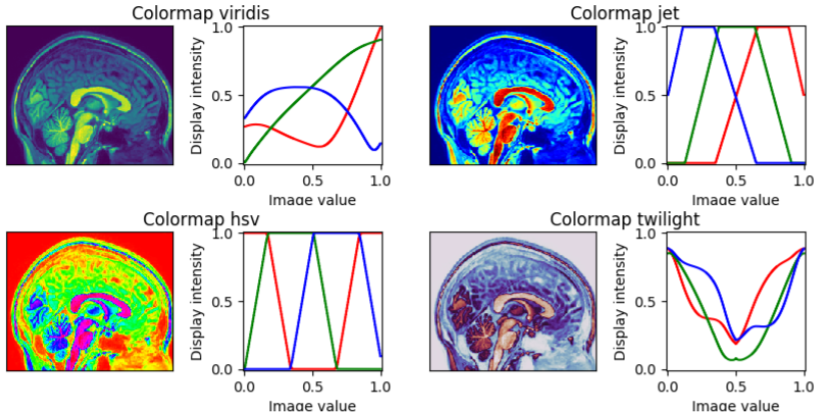
\includegraphics[scale=0.8]{W1_9.png}
\end{center}
\begin{itemize}
    \item Grayscale images can be mapped to colors to emphasize certain details.
    \item We chose 3 functions from [0, 1] $\rightarrow$ [0, 1], one for red, green, and blue.
    \item Colormap Jet is not perpectually uniform, and it is used for highlighting.  Often, Red = Bad, Blue = Good/Normal
    \item Color HSV is a "cyclic" colormap.  For this one, only Hue changes, while Saturation and Value stay constant.
    \item Colormap Twilight is a "diverging" colormap.  For this one, the "normal" is at 0.5, and the colors at that point are not altered.  Since lower values are mapped to red and higher values to blue, it shows the direction and magnitude of differences compared to the median.
\end{itemize}
Images with a signal value that is more than one dimension can be rendered as a color image by mapping different dimensions to the red, green, or blue channel.  The most common such type is a RGB image, which stores color values directly, but there are other possibilities.  For example, it is sometimes useful to display multiple images on top of one another, to see how signals co-localize in different images.  One image can be set to green, and one to magenta, as shown in the figure below
\begin{center}
    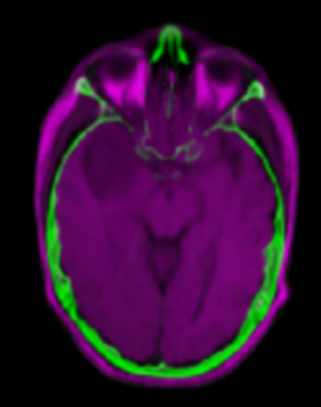
\includegraphics[scale=1]{W1_10.png}
\end{center}
\begin{itemize}
    \item This type of image is used to show complementary data.
    \item This image in particular maps the MRI scan to red + blue, and CT scan is green.
\end{itemize}
\subsection*{Code for Multimodal Images}
\begin{minted}{python3}
    import numpy as np
    import matplotlib.pyplot as plt
    # ...
    # I is a 2D array storing grayscale MR data,
    # normalized to the range [0,1]
    # J is a 2D array storing grayscale CT data,
    # normalized to the range [0,1]
    f,ax = plt.subplots()
    RGB = np.concatenate((I,J,I), axis=-1)
    ax.imshow(RGB)
\end{minted}
\subsection*{Feature Maps}
\begin{itemize}
    \item Feature maps such as texture classifiers can be mapped to RGB channels to visualize high dimensional data.
\end{itemize}
\begin{center}
    \includegraphics*[width=\textwidth]{W1_11.png}
\end{center}
\section*{3D Images}
\begin{itemize}
    \item Unlike natural images, most medical imaging data is 3D.
    \item In the absense of virtual reality platforms, these must be represented in 2D.
\end{itemize}
\subsection*{Slice directions}
\begin{center}
    \includegraphics*[width=\textwidth]{W1_12.png}
\end{center}
\begin{itemize}
    \item Coronal plane is an image taken from the front/back.
    \item Sagittal plane is an image taken from the left/right side.
    \item Axial plane is an image taken from the top/bottom.
\end{itemize}
\subsection*{Linear Projections}
\begin{itemize}
    \item Let $J(x, y) = \int I(x, y, z) \text{d}z$
    \item In Python, this can be implemented as \texttt{J = np.sum(I, axis=2)}.
    \item We are essentially summing all the pixels on one axis.  We can generate three projections since there are three axes we can sum over.
    \item Linear projections can simulate a radiograph
\end{itemize}
\begin{center}
    \includegraphics*[width=\textwidth]{W1_13.png}
\end{center}
\subsection*{Maximum Intensity Projection}
\begin{itemize}
    \item Let $J(x, y) = \text{Max} I(x, y, z)$
    \item In Python, \texttt{J = np.max(I, axis=2)}.
    \item Here, we take the maximum of each pixel over an axis.  Like linear projections, we can create three projections since there are three axes we can sum over.
    \item MIPs are often useful for thin structures like vessels.
    \begin{itemize}
        \item In a slice, vessels look like a dot.
        \item In a linear projection, vessels are obscured by everything else.
        \item Same goes with neuron axons, etc.
    \end{itemize}
\end{itemize}
\begin{center}
    \includegraphics*[width=\textwidth]{W1_14.png}
\end{center}
\subsection*{Isosurfaces}
\begin{itemize}
    \item By selecting a threshold, we can draw a surface that separates bright regions from dark regions.  Below, two thresholds are shown.
\end{itemize}
\begin{center}
    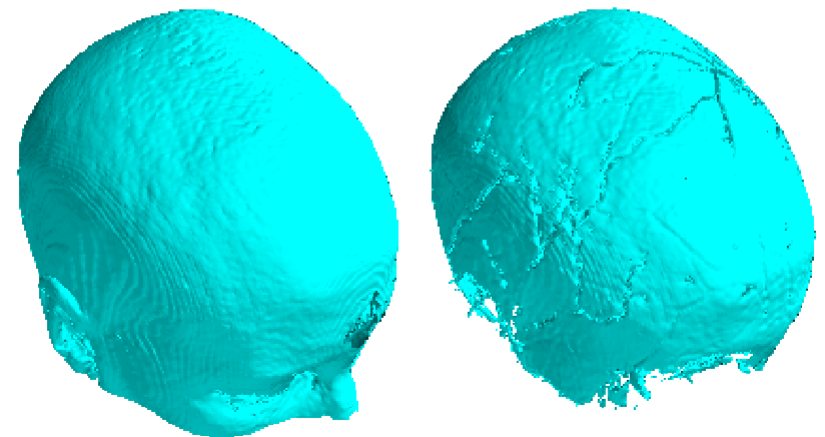
\includegraphics[width=\textwidth]{W1_15.png}
\end{center}
\begin{itemize}
    \item This is like a topography image.  In topography, changes in altitude on a mountain is viewed as circles.  In an isosurface, we are doing this in 3D.  The boundary created is a difference in brightness.  As such, one side of the boundary is brighter than the threshold, the other side is darker.
\end{itemize}
\subsubsection*{Isosurface Code}
\begin{itemize}
    \item Matpoltlib is not good at rendering 3D data, like isosurfaces.  One alternative in Python is mayavi.
\end{itemize}
\begin{minted}{python3}
    from mayavi import mlab
    # ...
    # I is a 3D array storing grayscale imaging data
    mlab.init_notebook()
    f = mlab.figure(bgcolor=(1.0,1.0,1.0),fgcolor=(0.0,0.0,0.0))
    mlab.contour3d(I,contours=[20.0], color=(0.0,1.0,1.0))
\end{minted}
\begin{itemize}
    \item The best way to explore 3D data is with interactive software.
    \item Examples:
    \begin{itemize}
        \item ITKsnap
        \item Paraview
        \item Imaris
    \end{itemize}
\end{itemize}
\end{document}
